\chapter{Stand der Technik}

\section{Virtuelle Realität}
Boas definiert in  seiner Arbeit \cite{Boas2012} Virtuelle Realität (VR) als ein Feld der Computerwissenschaften mit dem Ziel, immersive virtuelle Welten zu erschaffen und dem Benutzer die Möglichkeit geben, mit dieser Welt zu interagieren. 
Da die reale Welt hauptsächlich von unseren Sinnen und den Konsequenzen unseres Handelns wahrgenommen wird, entsteht durch die Simulation dieser Phänomene eine Virtuelle Umgebung (VU). Dazu muss für einen oder mehrere unserer Sinne ein alternativer Stimulus präsentiert werden. Zusätzlich müssen die Bewegungen und Aktionen des Benutzers in Betracht gezogen werden und die VU muss entsprechend darauf reagieren.
Durch die alternativen Stimuli und die Reaktion der VU auf die Aktionen des Benutzers entstehen zwei grundsätzliche Anforderungen an das System im Zusammenhang mit dem Benutzer. Der Mensch besitzt im übertragenen Sinn wie ein Computer Schnittstellen zur Eingabe und Ausgabe. Die Eingabeschnittstellen des Menschen sind die Sinne, deshalb muss das System Informationen ausgeben, die die Sinne stimulieren. Das häufigste Beispiel dafür ist die Ausgabe von Informationen über einen Bildschirm, welche von den Augen aufgenommen und im Gehirn verarbeitet werden. Die Ausgaben eines Menschen sind die Aktionen, die er ausführen kann. Zu den Aktionen gehören z. B. Sprache oder Bewegungen. Je mehr Ausgaben eines Menschen das System als Eingabe annimmt, desto realistischer wirkt die VU. Beispiele dafür wären Spracherkennung oder die Möglichkeit durch Bewegungen mit der VU zu interagieren.
Holloway\cite{Holloway1995} hat in seinem Paper im Jahr 1995 eine Tabelle erstellt, die für jeden menschlichen Sinn eine Methode der Stimulation beschreibt. Darin kommen nicht nur die klassischen fünf Sinne des Menschen Hören, Schmecken, Riechen, Sehen und Tasten vor, sondern auch weitere Empfindungen wie die Bewegungsempfindung (Kinästhetik), die Wahrnehmung der Körperbewegung und -lage im Raum (Propriozeption) sowie der Gleichgewichtssinn.
Eine weitere Tabelle stellt verschiedene Geräte vor, die die Bewegungen und Aktionen des Benutzers erfassen können. Zu den Aktionen gehören Kopfbewegungen, Bewegungen des Körpers und Gliedmaßen, Fingerbewegungen, Ausrichtung der Augen, Sprache und Ausübung von Kräften.
Aktuelle Verbraucher basierte VR-Brillen fokussieren sich in der Regel auf den Sehsinn und Hörsinn, da es sich herausgestellt hat, dass diese Sinne am einfachsten permanent virtualisiert werden können. Das zeigt sich auch an normalen Computern, die in der Regel über Bildschirme und Lautsprecher verfügen.\cite{Holloway1995}

Aus den genannten Gründen ist der Klassische und am meisten verfügbare Weg VR zu erleben ein Head-Mounted Display (HMD), ein Gerät, welches um den Kopf geschnallt wird und komplett die Augen verdeckt. HMDs haben in der Regel stereoskopische Bildschirme um 3D Welten in einem großen Blickfeld darzustellen. Jeder der Bildschirme befindet sich jeweils genau vor einem Auge, was die künstliche Stimulation der visuellen Wahrnehmung ermöglicht. Viele HMDs haben die Möglichkeit, die Distanz zwischen den beiden Bildschirmen an die Distanz zwischen den Augen verschiedener Benutzer anzupassen. Für die wirkliche dreidimensionale Illusion werden in der Software zwei Kameras, eine für jedes Auge, eingebunden und entsprechend platziert.
Die Simulation der auditiven Wahrnehmung kommt ebenfalls oft zum Einsatz. Da HMDs in der Regel an einen Computer angeschlossen werden müssen und diese grundsätzlich die Kapazitäten für ein Lautsprechersystem besitzen, ist es der Standard, dass VR Anwendungen mithilfe der Lautsprecher Geräusche und Musik verwenden. Alternativ ist die Verwendung von Kopfhörern möglich, da diese im Gegensatz zu Lautsprechern nur die Geräusche der VU zulassen und alle realen Geräusche unterdrücken, was zu höherer Immersion führt. Die Stimulation des Tastsinns beschränkt sich bei den meisten Verbraucher basierten Anwendungen auf Vibration der Controller bei bestimmten Situationen. Es existieren bereits kommerzielle Geräte, die sich auf die virtuelle Stimulation des Tastsinns sowie auf die Kinästhetik fokussieren. Sogenannte \textit{Haptic Gloves}, zu Deutsch haptische Handschuhe können Berührungen, verschiedene Oberflächen und Force Feedback (Kraftrückkopplung) simulieren. Aufgrund des Größenunterschiedes verschiedener Hände sind die Haptic Gloves noch nicht weit verfügbar \cite{Perret2018}.

Von den von Holloway \cite{Holloway1995} gelisteten Aktionen, die erfasst werden sollen, ist es mittlerweile technisch gesehen möglich, alle zu erfassen.
Durch Gyroskope und Beschleunigungssensoren erkennt das Headset die Ausrichtung des Kopfes und kann entsprechend die Kameras in der Anwendung rotieren. Bei manchen Ausführungen wird auch die Position des Headsets und anderen Trackern durch Kameras erfasst. Dadurch kann sich der Benutzer durch Bewegungen im echten Raum im virtuellen Raum bewegen. \cite{Boas2012}\cite{Holloway1995} Bei der HTC Vive beträgt die maximale Raumgröße beispielsweise 6m x 6m.
Aktuelle VR Kits wie die HTC Vive oder die Oculus Rift werden standardmäßig neben dem HMD mit zwei Controllern ausgeliefert. Diese verfügen ebenfalls über tracking Kapazitäten, wodurch ihre Position im Raum identifiziert werden kann. Der Nutzer kann mit den Controllern eine Reihe von Interaktionen Ausführen. Die Interaktionen reichen von einfachen Aktionen wie Aufheben und Werfen von Objekten bis zu komplexen Aufgaben wie das Spannen und Abfeuern eines Bogens oder das Zusammensetzen eines Puzzles. Verbraucher orientierte HMD Modelle in höheren Preisklassen bieten auch die Möglichkeit zur Erfassung der Augenbewegungen. Dazu sind innerhalb des HMD Kameras angebracht, die die Rotation der Augen erfassen. Spracherkennung ist ebenfalls ein gut erforschtes Thema und es gibt bereits eine Anzahl an Spielen und Anwendungen die auf Sprachsteuerung basieren. \cite{Lamberti2017} 

VR beschränkt sich nicht nur auf die Forschung und Unterhaltungsbranche, sondern wurde bereits erfolgreich in verschiedenen anderen Anwendungsgebieten eingesetzt. Vor allem Trainingsumgebungen im Militär oder in der Medizin profitieren von der Immersiven Umgebung und den vielseitigen Interaktionen von VR Systemen. Weitere Beispiele für VR Anwendungsgebiete sind Fahr- und flugsimulationen, welche den kompletten Fahrzeugraum simulieren können und so ein realistisches Trainingsumfeld ohne Risiken bieten.\cite{Ragan2010}
 

\section{Immersion}
Slater\cite{Slater2003}\cite{Slater1999} definiert Immersion objektiv als die Technologischen Kapazitäten eines Systems. Je mehr verschiedene Sinne ein System durch virtuelle Reize stimuliert und je genauer die Erfassung der Aktionen des Benutzers und deren Übertragung in die VU ist, desto immersiver ist das System. Dadurch kann laut Slater Immersion objektiv bewertet und theoretisch gemessen werden und hat nichts damit zu tun, wie verschiedene Menschen Immersion wahrnehmen. Trotzdem kann jeder dasselbe immersive System unterschiedlich Wahrnehmen und unterschiedliche Reaktionen darauf haben. Slater nennt diese menschliche Reaktion auf Immersion Presence (Präsenz, Anwesenheit) und betont in seinen Arbeiten die starke Abgrenzung von Immersion und Presence. Als Analogie verwendet er Farben. Immersion ist dabei analog zur Verteilung von Wellenlängen, die alle Farben abgeben, was objektiv gemessen und beschrieben werden kann. Jeder Mensch nimmt aber Farben unterschiedlich wahr und hat verschiedene emotionale Reaktionen auf jede Farbe als andere Menschen. Somit ist das Konzept der Präsenz analog zur Wahrnehmung von Farben. Presence beschreibt also die Beziehung zwischen einem selbst und der Umgebung.
Bowman und McMahan\cite{Bowman2007} gehen bei der Definition von Slater einen Schritt weiter und fokussieren sich bei der Messung von Immersion am Grad der Visuellen Immersion, auch wenn sie nur ein Teil der gesamten Immersion eines Systems ist. Dabei hebt er die rendering Software sowie die Bildschirmtechnologie vor. Seine wichtigsten Faktoren für Visuelle Immersion beinhalten beispielsweise die Auflösung und Größe eines Bildschirms, field of View sowie die Frame Rate.
Ein potenzieller Vorteil eines höheren Grades an Immersion ist das räumliche Bewusstsein. In der realen sowie der virtuellen Welt nehmen wir dauerhaft eine dreidimensionale Umgebung wahr, obwohl unsere Augen nur zweidimensionale Bilder aufnehmen. Das liegt daran, dass unser Gehirn stark darauf Optimiert ist, eine dreidimensionale Umgebung mithilfe von Stereopsis, Bewegungsparallaxen, Perspektive und Okklusion zu rekonstruieren. 
Immersive VR liefert künstliche Stimuli für all diese Tricks, die unser Gehirn verwendet. Stereopsis, also Stereoskopisches Sehen wird durch die beiden Bildschirme in den HMDs und den beiden Kameras in der Anwendung ermöglicht. Bewegungsparallaxe können sowohl in 2D als auch in 3D Umgebungen z.B. durch Parallax-Scrolling simuliert werden. Dabei handelt es sich um den optischen Effekt, wenn verschiedene Objekte unterschiedlich weit voneinander entfernt sind, und der Beobachter sich horizontal dazu bewegt. In dreidimensionalen virtuellen Welten ist dieser Effekt bereits von Natur aus gegeben. Okklusion, also der Effekt, wenn näher gelegene Objekte weiter entfernte Objekte verdecken, sowie Perspektive sind in den meisten normalen 3D Anwendungen ebenfalls bereits gegeben und sind nicht VR spezifisch.
Das durch die genannten Tricks verstärkte räumliche Bewusstsein, kann zu größerer Effektivität in Anwendungen wie Wissenschaftlicher Visualisierung, Design Reviews und Virtuellen Prototypen von 3D Objekten dienen.

\section{Presence}
Presence und embodiment werden verwechselt
selbst der term embodiment ist nicht immer einheitlich aufgefasst \cite{Kilteni2012}
Embodiment ist eher körperbezogen
Sense ofEmbodiment1 (SoE) will be used to refer to the ensemble ofsensations that arise in conjunction with being inside, having, and controlling a body2 especially in relation to virtual reality applica- tions

Slater\cite{Slater2003}\cite{Slater1999}
Abgrenzung von Immersion und Embodiment
3 aspekte von presence
The sense of ‘being there’ in the environment depicted by the VE. • The extent to which the VE becomes the dominant one - i.e., that participants will tend to respond to events in the VE rather than in the ‘real world’.
• The extent to which participants, after the VE experience, remember it as having visited a ‘place’ rather than just having seen images generated by a computer.


bei embodiment muss irgendwas wie ein körper vorhanden sein, presence kann man auch schon beim film schauen spüren

https://ispr.info/about-presence-2/about-presence/

\section{Self Embodiment}
abgrenzung zu presence
Embodiment kann als Verkörperung übersetzt werden. Damit ist gemeint, dass dem Benutzer ein passendes Selbstbild bereitgestellt wird um ihn für sich selbst und, in kollaborativen Situationen, für andere zu repräsentieren. Die Relevanz des Embodiments in VUs ist analog zur Relevanz des eigenen Körpers in alltäglichen Situationen. Unsere Körper liefern unserer Umgebung umgehend Informationen, wie unsere Anwesenheit, Aktivitäten, Aufmerksamkeit, Verfügbarkeit, Stimmung, Standort, Fähigkeiten und viele andere Faktoren. Der Benutzer kann mit seinem Körper durch Gesten und Körpersprache indirekt oder durch Zeichensprache in bestimmten Fällen direkt kommunizieren. \cite{Benford2010}
Ein mögliches Konzept des Embodiments ist, dass das Bewusstsein, einen Körper zu besitzen, die Erfahrungen aller Menschen grundlegend beeinflusst, egal ob dieser Körper physisch vorhanden ist oder nicht.\cite{Tham2018} Kilteni et al. \cite{Kilteni2012} geben in ihrer Arbeit an, dass das Nutzen von immersivem VR die Frage aufwirft, ob es möglich ist, dieselben Sinneseindrücke mit einem virtuellen Körper wie mit dem eigenen biologischen Körper zu fühlen und wenn ja, in welchem Ausmaß. Sie lassen sich  dabei von Forschung inspirieren, die sich mit Embodiment von künstlichen Körperteilen und Prothesen auseinandersetzt, indem sie diese Konzepte zu kompletten künstlichen Körpern erweitern. Zusammenfassend besagt ihre Definition von Embodiment, dass ein Objekt Embodied ist, also verkörpert wird, wenn manche Eigenschaften des Objekts subjektiv wie die Eigenschaften des eigenen biologischen Körpers behandelt werden und so das Gefühl auslöst, einen Körper zu besitzen.
Weiter definieren Kilteni et al., dass das Gefühl des Embodiments sich in drei Unterelemente aufteilen lässt. Erstens, das Gefühl, den eigenen Standort zu kennen(self-location).  Dies grenzt sich von der Erfahrung von Presence davon ab, dass die self-location nicht die Position innerhalb eines Raums beschreibt, sondern in welchem Körper man sich befindet. Zweitens, das Gefühl der Entscheidungsfreiheit (Agency). Agency verweist auf das Gefühl, motorische Kontrolle über den eigenen Körper zu haben. Das Gefühl der Agency ist beispielsweise gegeben, wenn man seinen eigenen Arm jederzeit willentlich bewegen kann. Ein Gegenbeispiel, bei dem die Agency gestört wird, ist das unbeabsichtigte Schütteln der Hände bei Parkinson Patienten. Das Dritte Unterelement ist Body Ownership, was das Gefühl beschreibt, einen eigenen Körper zu besitzen. Es hat einen besitzergreifenden Charakter und impliziert, dass der Körper die Quelle der gefühlten Empfindungen ist. Ein Beispiel dafür ist die Gummihand-Illusion. Dabei wird der echte Arm eines Menschen abgedeckt und an seiner Stelle ein Gummiarm platziert. Der reale Arm und der Gummiarm werden dann z. B. mit einem Pinsel gleichzeitig stimuliert. Testpersonen gaben nach dem Experiment an, nach einer Zeit der Stimulation nicht den versteckten Pinsel, sondern den Pinsel, den sie gesehen haben, spürten.\cite{Botvinick1998} Slater et al. \cite{Slater2008} führten ein an die Gummihand-Illusion angelehntes Experiment in VR mit Erfolg durch.


\section{Avatare}
Avatare sind digitale Repräsentationen von uns selbst. Ihre Darstellung variiert stark abhängig vom Kontext in dem sie eingesetzt werden. Sie reichen von einfachen Zeichnungen oder Bildern, die den Benutzer darstellen, wie es manchmal in Social Media zur Kommunikation eingesetzt wird, bis zu detailreichen, komplett ausgearbeiteten 3D Modellen, welche perfekt auf die jeweilige Person zugeschnitten sind und z. B. in High-End Simulationen zu finden sind.
Die äußere Erscheinung des Avatars hat großen Einfluss auf das Embodiment. Erscheinungsmerkmale wie Gestalt, Hautfarbe, Alter und Geschlecht als auch Art der Kleidung haben Einfluss auf die stärke der Embodiment Illusion, schließt die Möglichkeit auf Embodiment aber nicht aus. Sobald die Illusion des Embodiments gegeben ist, kann die Art des Avatars großen Einfluss auf das Verhalten einer Person haben. Ein Beispiel dafür sind verminderte Hautfarben bezogene Vorurteile, wenn hellhäutige Teilnehmer einen dunkelhäutigen Avatar Verkörpert haben. Verkörperung von kleineren oder größeren Avataren hat Einfluss auf die Fähigkeit selbstbewusst zu verhandeln. Selbst die Kleidung des Avatars kann Auswirkungen haben. Kilteni et. al haben in\cite{Kilteni2013} den Teilnehmern entweder einen lässig gekleideten dunkelhäutigen oder einen formal gekleideten hellhäutigen Mann eine afrikanische Handtrommel spielen lassen. Ihre Ergebnisse zeigen, dass die Erscheinung des Avatars großen Einfluss das Verhalten des Teilnehmers hat. Eine weitere Erkenntnis war, dass trotz der Männlichen Avatare das Geschlecht der Teilnehmer keinen Einfluss auf das Embodiment hatte.
Eine weitere wichtige Eigenschaft für Avatare neben der Darstellung ist die Kontrolle, die der Nutzer über den Avatar hat. Die Kontrolle reicht wie die Darstellung von komplett passiv und uninteraktiv wie bei Bildern bis zu dynamischen und komplett kontrollierbaren Avataren wie es oft in Computerspielen zu sehen ist. Je höher die Kontrolle über den Avatar ist, desto höher ist die Immersion und somit auch das mögliche Embodiment, welches der Nutzer erleben kann. Vor allem die Kategorie der Agency von Embodiment ist davon betroffen, da eine Aktion des Nutzers bei hoher Kontrollierbarkeit durch direkte Verknüpfung mit dem Avatar eine Aktion des Avatars auslöst.\cite{Biocca2014} Mohler et al. beschreiben in \cite{Mohler2010} das Avatare nicht immer für Embodiment sorgen. In ihrem Experiment befindet sich der Avatar des Nutzers drei Meter entfernt, lässt sich aber komplett steuern. Sie schließen die Möglichkeit des Embodiments trotzdem nicht aus, da die Agency durch die Kontrolle gegeben ist.
Obwohl die Forschung zeigt, dass Avatare signifikanten Einfluss auf das mögliche Embodiment hat, setzen vergleichsweise wenige HMD-basierte VR-Systeme Avatare ein, die den kompletten Körper repräsentieren \cite{Pan2017}.

\section{Kinematik}
Eine gängige Methode um Avatare zu animieren, damit der Nutzer einen hohen Grad an Kontrolle darüber hat, ist über inverse Kinematics. Kinematik ist ein Feld der Mechanik, wobei der Körper als Zusammensetzung von Verbindungen dargestellt wird. Dabei bleiben andere Attribute wie Kraft und Masse unberücksichtigt. In der Computeranimation werden dafür sogenannte Knochen eingesetzt, welche wiederum aus Gelenken bestehen. Jeder Knochen wirkt sich auf die umliegende Fläche unterschiedlich aus und lässt sich an dem Gelenk bewegen, wodurch der beeinflusste Teil des Körpers mit bewegt wird.
Die Methodik der Kinematik beinhaltet die Vorwärtskinematik und die Inverse Kinematik. Wenn die Winkel aller Gelenke gegeben sind und die Position und Rotation der Segmente berechnet werden müssen, kommt die Vorwärtskinematik zum Einsatz. Wenn wiederum die Position und Rotation der Gelenke gegeben ist, und die Winkel ausgerechnet werden müssen, kommt die Inverse Kinematik zum Einsatz. Der Fall der Inversen Kinematik ist bei der Animation von Avataren in VR gegeben. Wenn z. B. die Position und Rotation der Controller bekannt ist, jedoch keine weiteren Informationen über den Arm des Benutzers vorliegen, muss berechnet werden, wie der Arm des Avatars angewinkelt ist und wo sich der Ellbogen befindet.\cite{Xia2009}
Um Avatare mit IK zu animieren, muss ein sogenanntes Rig, also ein Skelett, für den Avatar gegeben sein. Dabei werden die einzelnen Teile eines Meshes(Polygonnetzes) an einzelne Knochen des Rigs gekoppelt. Werden die Knochen bewegt oder rotiert, bewegt sich der zugewiesene Teil des Rigs ebenfalls entsprechend.
\begin{figure}[h]
  \makebox[\textwidth]{
    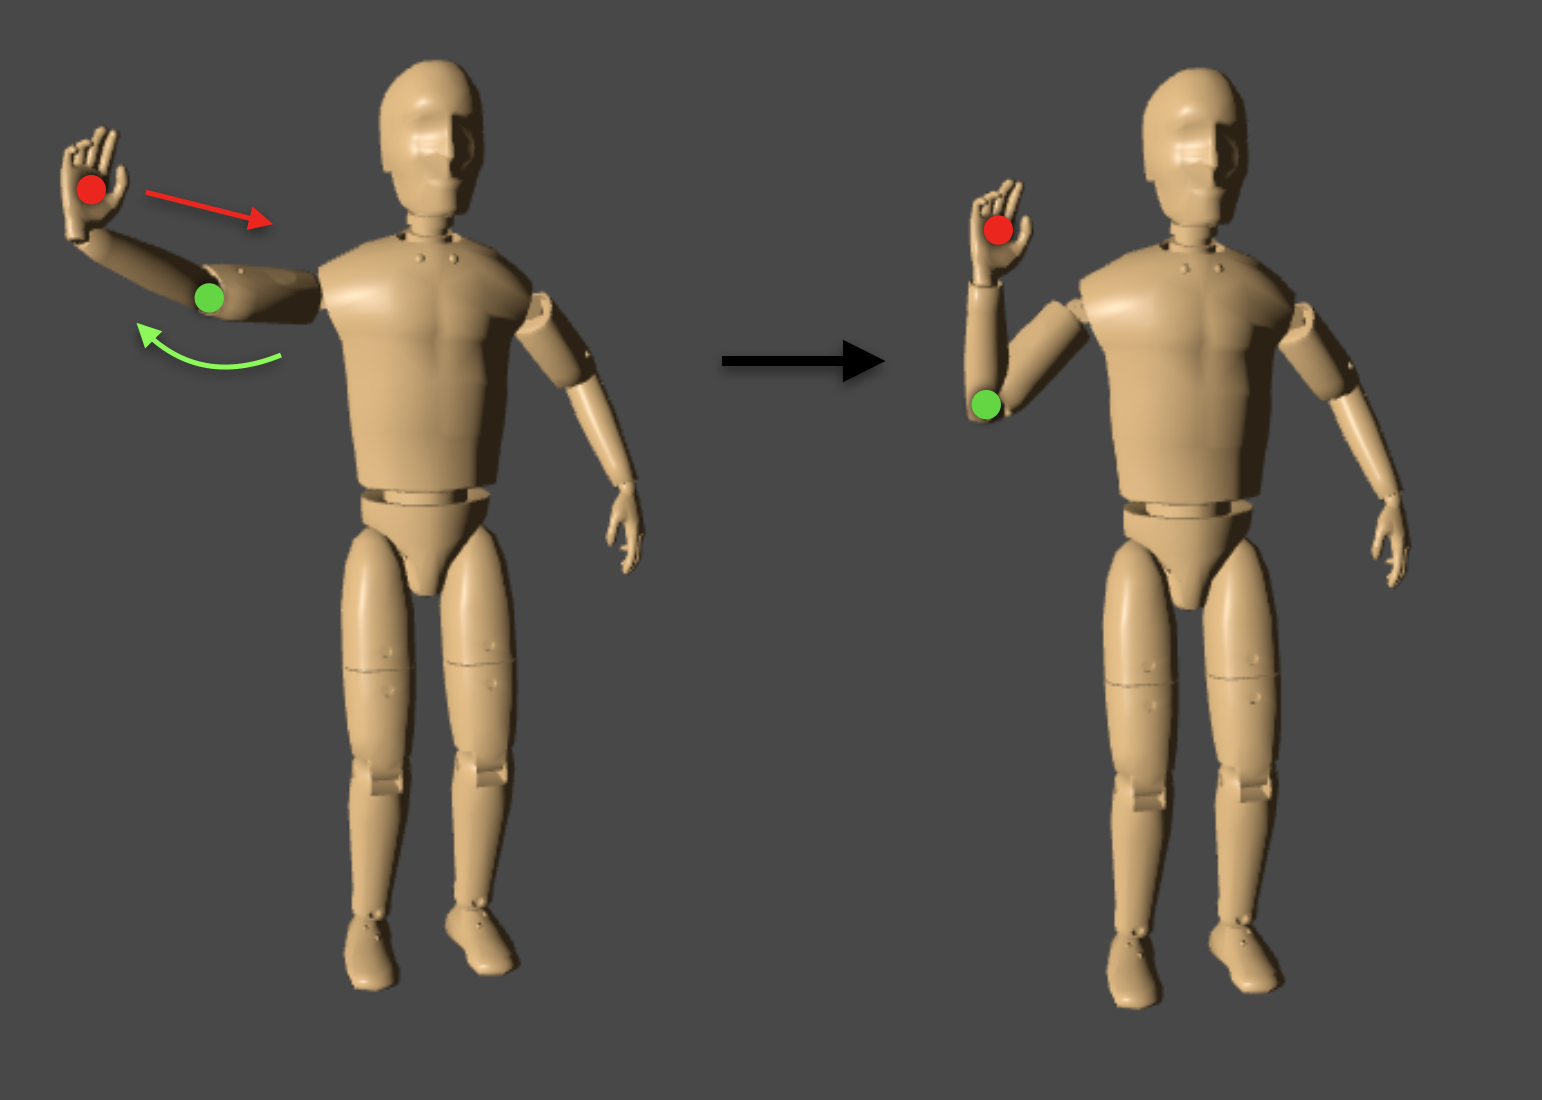
\includegraphics[width=\textwidth]{Bilder/Game/IKDummiesPicture.png}
  }
  \caption[Inverse Kinematik am Beispiel Dummy]{Inverse Kinematik am Beispiel Dummy.}
  \label{fig:IKDummy}
\end{figure}
Abbildung \ref{fig:IKDummy} zeigt einen Anwendungsfall von IK anhand des Dummies, der in dem Versuch eingesetzt wird. Der Dummy stammt aus dem Demobeispiel VRIK aus der Bibliothek FinalIK. Das Beispiel zeigt eine einfache Bewegung einer erhobenen Hand, im Bild durch den roten Pfeil dargestellt.
Dabei wird davon ausgegangen, dass die Position der Hand, die im Bild durch die roten Punkte dargestellt wird, dem System bekannt ist. Die im Bild grünen Punkte zeigen das sogenannte \textit{Bend Goal}. Ein Bend Goal ist ein Gelenk, welches durch Einflüsse eines Endpunktes bewegt wird. Die Position des Bend Goals ist dem System nicht bekannt, die Aufgabe des IK ist es, die Position und den Winkel des Bend Goals auszurechnen. Beispiel Wie?


\section{Motion Tracking}


\section{Stand der Wissenschaft}
agency hat auswirkungen auf embodiment: \cite{Koilias2019}

Kollias hat rausgefunden:
Agency hat keine auswirkungen auf body ownership
große unterschiede wenn Körper bewusst angeschaut wird, und vor einem Spiegel
schon allein wenn man läuft sind keine unterschiede zu erkennen











